\chapter{Multidimensional grids and data}
The dimensions of the grid(containing blocks) and blocks(containing threads) is given by the built-in variables, \textbf{\texttt{gridDim}} and \textbf{\texttt{blockDim}} variables. These parameters are specified within the \textit{execution configuration parameters, $<<<\dots>>>$} of the kernel call statement.\\\texttt{$<<<$ dimGrid, dimBlock $>>>$}
\begin{itemize}
    \item
          \begin{center}
              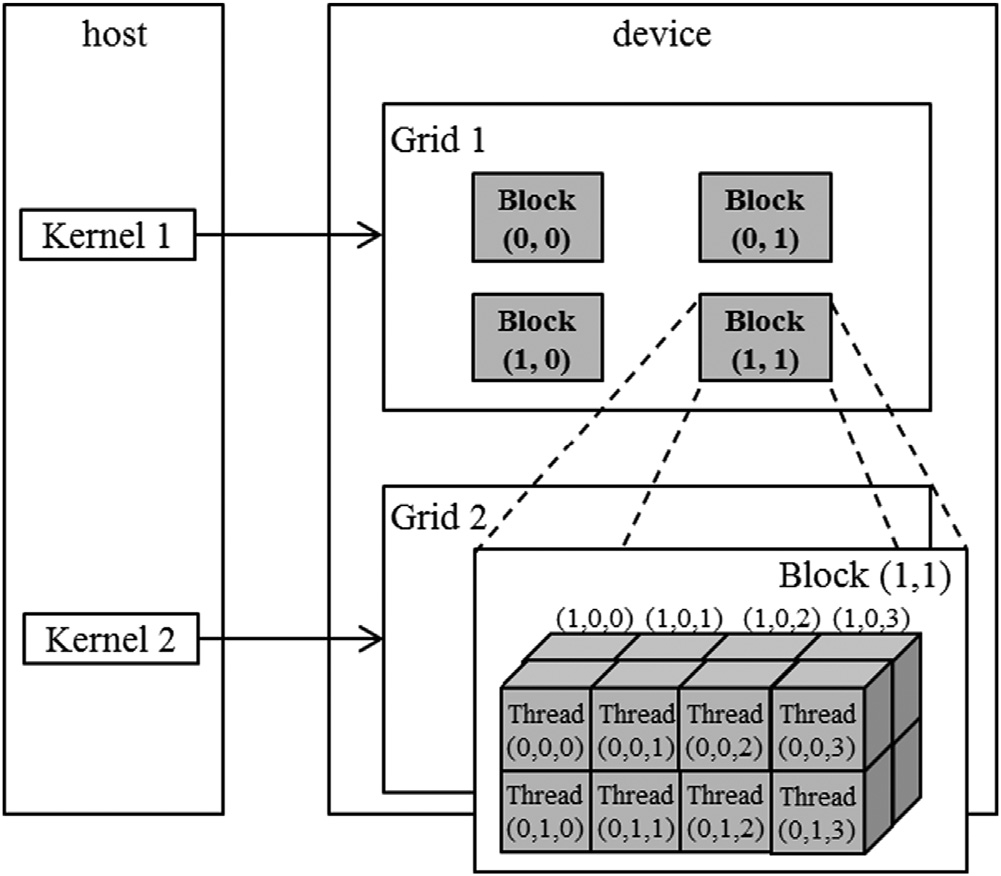
\includegraphics[width=0.6\linewidth]{Images/MultiDim_Grid/grid_structure.png}
          \end{center}
    \item \textbf{Grid }$\rightarrow$ 3D array of blocks.
          \begin{itemize}
              \item All blocks share the same \texttt{gridDim.x, gridDim.y, gridDim.z} values.
          \end{itemize}
    \item \textbf{Block} $\rightarrow$ 3D array of threads.
          \begin{itemize}
              \item All threads in a block share the same \texttt{blockIdx.x, blockIdx.y, blockIdx.z} values.
              \item Total number of threads in a block is constrained to 1024 and can be distributed flexibly in the 3 dimensions.
              \item \texttt{blockIdx.x} $\in \{0 \dots \texttt{gridDim.x - 1} \}$\\\texttt{blockIdx.y} $\in \{0 \dots \texttt{gridDim.y - 1} \}$\\\texttt{blockIdx.z} $\in \{0 \dots \texttt{gridDim.z - 1} \}$
          \end{itemize}
    \item \textbf{Thread} $\rightarrow$ Has \textbf{unique identifier} in a block.
          \begin{itemize}
              \item \texttt{threadIdx.x} $\in \{0 \dots \texttt{blockDim.x - 1} \}$\\\texttt{threadIdx.y} $\in \{0 \dots \texttt{blockDim.y - 1} \}$\\\texttt{threadIdx.z} $\in \{0 \dots \texttt{blockDim.z - 1} \}$
          \end{itemize}
\end{itemize}

\begin{minted}{cpp}
    // 1D grid with 32 blocks in x direction.
    dim3 dimGrid(32, 1, 1);
    // 1D block with 128 threads in x direction.
    dim3 dimBlock(128, 1, 1);
    // Kernel call
    vecAddKernel<<<dimGrid, dimBlock>>>(...);
    // Shorthand convention
    vecSubKernel<<<32, 128>>>(...);
\end{minted}

\section{Linearization of 2D array}
The main two ways in which a 2D array can be linearized, \textit{row-major layout} and \textit{column-major layout}. In \textbf{row-major layout}, the same elements of the same rows are placed into consecutive locations. The rows are placed one after other consecutively in memory space. An element at jth row and ith column is indexed as $M_{j, i}$. \textit{CUDA C uses the row-major layout.}
\begin{center}
    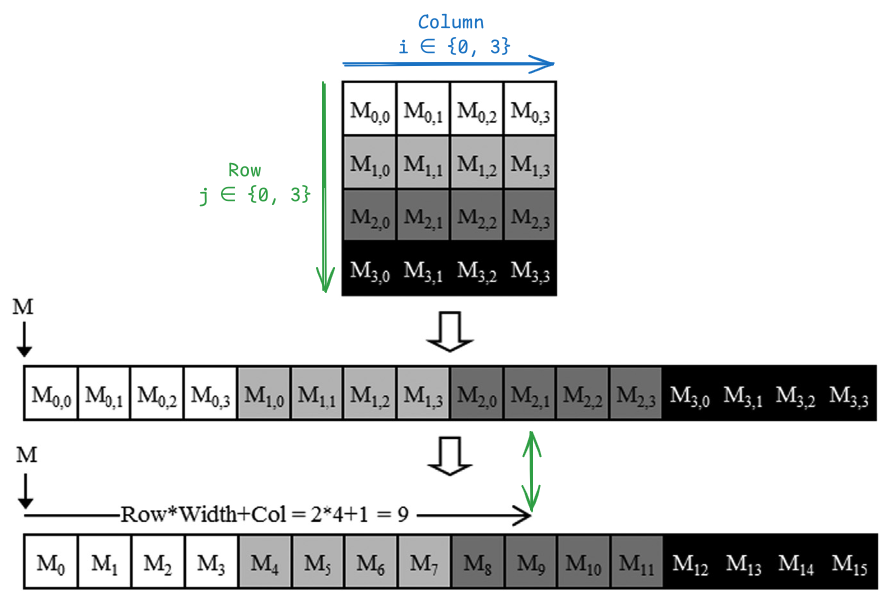
\includegraphics[width=0.7\linewidth]{Images/MultiDim_Grid/Linearizing_array.png}
\end{center}
\bigskip
The formula to convert an image from color to grayscale is described as:
\begin{center}
    $L = 0.21*r + 0.72*g + 0.07*b$
\end{center}

\begin{minted}{cpp}
    // The input image is encoded as unsigned chars [0, 255]
    // Each pixel is 3 consecutive chars for 3 channels (RGB)
    __global__
    void colortoGrayscaleKernel(unsigned char* Pout, unsigned char* Pin, 
                                            int width, int height) {
        int col = blockIdx.x * blockDim.x + threadIdx.x;
        int row = blockIdx.y * blockDim.y + threadIdx.y;

        if (col < width && row < height){
            // Get index of the current element of output
            int grayOffset = row * width + col;
            // RGB array has CHANNELS * elements of grayscale image.
            int rgbOffset = grayOffset * CHANNELS;
            // Red, Green and Blue values
            unsigned char r = Pin[rgbOffset];
            unsigned char g = Pin[rgbOffset + 1];
            unsigned char b = Pin[rgbOffset + 2];
            // Perform rescaling and store in the out array (Grayscale img)
            Pout[grayOffset] = 0.21f * r + 0.72f * g + 0.07f * b; 
        }
    }
\end{minted}
\bigskip
For an image of size 62 $\times$ 76, and block size in \textit{x, y} of (16, 16), the linearized 1D index of the \texttt{Pout} pixel at thread (0, 0) and block (1, 0) is calculated as:
\begin{equation*}
    \begin{aligned}
        \text{Pout}_{blockIdx.y *blockDim.y + threadIdx.y , blockIdx.x*blockDim.x + threadIdx.x} \\
        = \text{Pout}_{1*16+0, 0*16+0} = \text{Pout}_{16,0} = \text{Pout}[16*76+0] = \text{Pout}[1216]
        \\\end{aligned}
\end{equation*}

\section{Image blur Kernel}
\begin{center}
    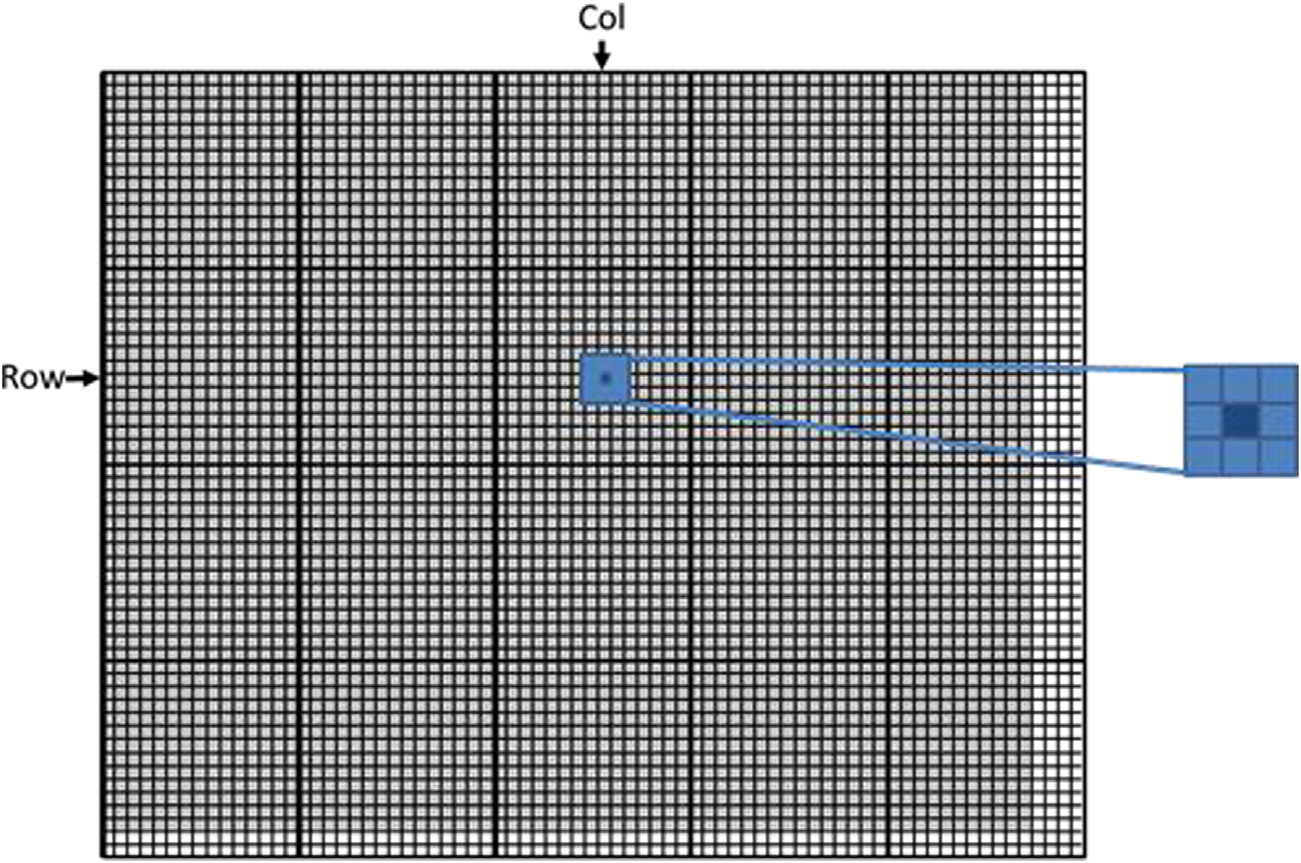
\includegraphics[width=0.6\linewidth]{Images/MultiDim_Grid/image_blur.png}
\end{center}
